\chapter{Theoretical framework} \label{framework}

To assess the various remote sensing techniques and damage classification methods, a theoretical framework has to be established. This framework will allow the organisation of methods and technologies and will allow the selection of appropriate approaches in various circumstances. The framework presented here is based on literature research from \citet{Dong2013} and \citet{Kerle2008} in combination with requirements from the field.

\section{Disaster}\label{sec:dis}
The International Federation of Red Cross and Red Crescent Societies \citeyearpar{IFRC2017} defines a disaster as follows: 
\begin{quote}
	\textit{"A disaster is a sudden, calamitous event that seriously disrupts the functioning of a community or society and causes human, material, and economic or environmental losses that exceed the community’s or society’s ability to cope using its own resources."}
\end{quote}
These characteristics in this definition emphasize the need for timely intervention by others outside a community or area to help and support those affected. Ray Shirkhodai notes in \citet[p. i]{AlAchkar2008} that a rapid overview of the situation and extent of damage is necessary to achieve this goal, as is corroborated by \citet{Okada2000} and \citet{Schweier2006}. This rhetoric is an abstract approach to the problem, in reality every step within the \ac{drm} cycle have separate requirements for information regarding to damage. The faster more detailed information is available, the better. However, the first phase of the \ac{drm}, Search and Rescue, requires much less detail for teams to be send into the field. This is a limitation set forward by the time necessary for the procurement of data and information. The result is a curve closely linked to time, in which the data detail requirements rise as time passes. This research focusses on the emergency relief and rehabilitation phase, towards recovery [figure \ref{fig:drm_cyc}] \citep{Wisner2002, Crutchfield2013}. In these first week after a disaster, the needs for information change from a course overview per area affected, to highly detailed information on a block or even building level \citep{Ozisik2004}.\\

\begin{figure}[!h]
	\centering
	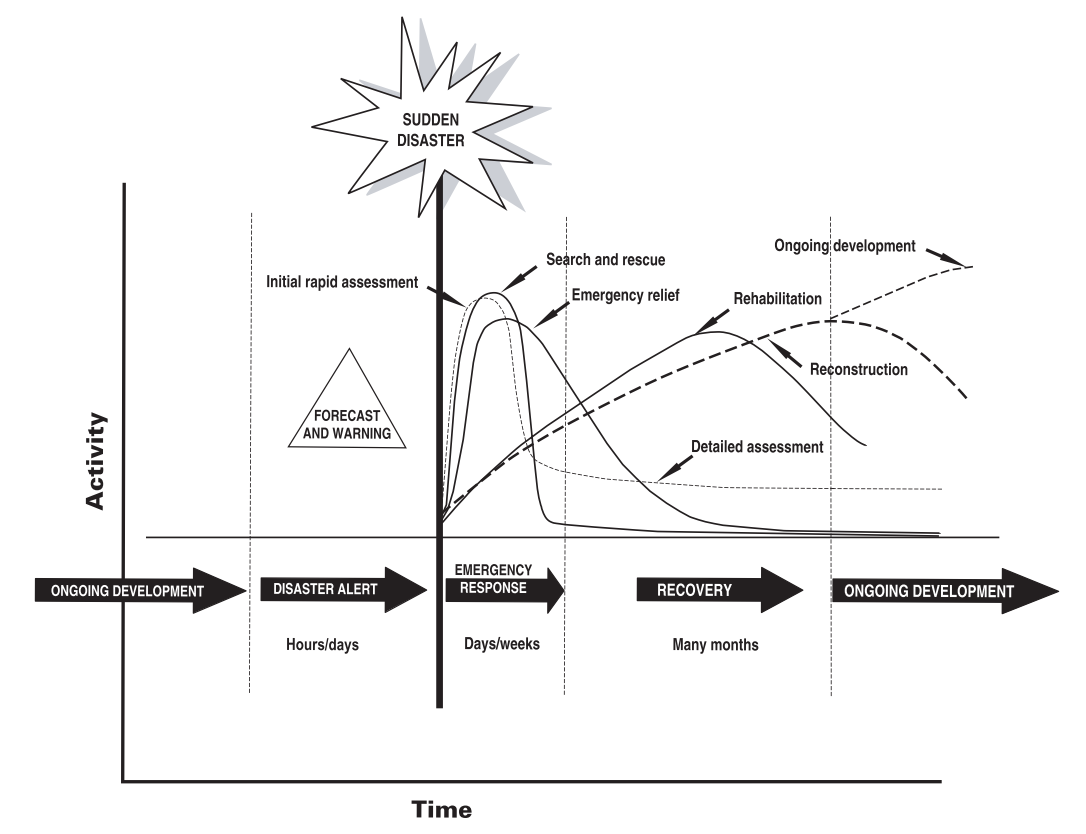
\includegraphics[width=0.65\textwidth]{figs/Drm_activity.png}
	\caption{\footnotesize{\ac{drm} activity cycle, including ongoing development. [From: \citet[p. 19]{Wisner2002}]}}
	\label{fig:drm_cyc}
\end{figure}

 \noindent To gather this data with minimum risk to aid workers, the international community established the so-called International Charter \citep{Bessis2003}. With resources from various space agencies around the world it became possible to use \ac{sem} to provide rapid situation awareness after a disaster. However, as described by \citet{Kerle2008} there are a diverse selection of other remote sensing techniques which can be used for the collection of data, which could make other forms of \ac{em} possible. This research will take into account this broader approach to remote sensing, looking at advances in \ac{uav} and shrinking data collection technologies as new data sources in the immediate aftermath of a disaster.

\section{Detection, Classification, and Assessment} \label{sec:clas}

Besides spatial resolution scales of information [house, block, neighbourhood], the results of \ac{em} can also be categorised in various information densities. For the purpose of this research these have been categorised as follows:

\begin{itemize}
	\item Damage detection
	\item Damage classification
	\item Damage assessment
\end{itemize}

\noindent The lowest information density considered is damage detection [figure  \ref{fig:Dam_Det}]. In this form of \ac{em} the focus is to differentiate between buildings with and without damage. This comparable to the studies that can distinguish between two grades of damage as described by \citet{Dong2013}. An example of this is \citet{Wang2012}, in which image classification is used to derive the difference between buildings damage and not damaged by a disaster.\\

\noindent One step up from detection is the damage classification as used within this research [figure  \ref{fig:Dam_Class}]. For classification, various grades of damage need to be considered. \cite{Dong2013} describe this as three grades or more. They also provide a framework for five damage classes that can be used in achieving damage classification. These classes are derived from \citet{Grunthal1998}, however the ambiguity introduced with five classes, especially between the three middle grades, is not beneficial for humanitarian aid organisations. Therefore, the classification method proposed by \citet{AlAchkar2008}, known as the \ac{bar}, will be used in this research. This framework is focused on damage inflicted to buildings, allows for sufficient variation between damage grades and has example of damage induced by wind. The four classes identified within the \ac{bar} method are: [1.] No visible damage, [2.] Minimal Damage, [3.] Significant Damage, and [4.] critical damage, examples of the damage extend are available in figure \ref{fig:Dam_Class} and \citet{AlAchkar2008}. A simplified variation of this is also used by the \ac{nlrc} and is used within this research due to the availability of data. [Simplified approach available on \href{https://www.510.global/visual-guide-damage-assesment/}{510.global}].\\

\noindent The last resolution is damage assessment [figure  \ref{fig:Dam_Ass}]. This requires more insight in the damage caused, as well as interior damage which is usually not observable in \ac{em} or \ac{sem}. Therefore people on the ground are required to do thorough investigation into the damage caused. The exception to this is the use of high resolution oblique imagery, which in some cases might be able to distinguish damage in the vertical plane \citep{Vetrivel2016a}, however most damage assessment will need to be done by humans with guides from governments, like from \citet{FEMA2016}.\\

\begin{figure}[!h]
	\centering
	\includegraphics[width=0.95\textwidth]{figs/Dam_Det.png}
	\caption{\footnotesize{Example of damage detection [Based on: Netherlands Red Cross (11 Sept. 2017), Cole Bay - Sint Maarten [georeferenced image], used under CC-BY4.0 as part of Open Imagery Network, retrieved from \url{www.openaerialmap.org}]}}
	\label{fig:Dam_Det}
\end{figure}
\begin{figure}[!h]
	\centering
	\includegraphics[width=0.95\textwidth]{figs/Dam_Clas.png}
	\caption{\footnotesize{Example of damage classification [Based on: Netherlands Red Cross (11 Sept. 2017), Cole Bay - Sint Maarten [georeferenced image], used under CC-BY4.0 as part of Open Imagery Network, retrieved from \url{www.openaerialmap.org}]}}
	\label{fig:Dam_Class}
\end{figure}
\begin{figure}[!h]
	\centering
	\includegraphics[width=0.95\textwidth]{figs/Dam_Ass.png}
	\caption{\footnotesize{Example of damage assessment [Based on: Netherlands Red Cross (11 Sept. 2017), Cole Bay - Sint Maarten [georeferenced image], used under CC-BY4.0 as part of Open Imagery Network, retrieved from \url{www.openaerialmap.org}]}}
	\label{fig:Dam_Ass}
\end{figure}

\subsubsection*{Classification}
Statistical classification is the methods for organising various samples in the right classes \citep{Theodoridis2009}. Humans are able to discern various features of an object to decide the classification. To achieve the same with the help of machine intelligence, various methods have been described. These range from linear classifiers to Support Vector Machines and Neural Networks. These can be subdivided in Supervised, Semi-Supervised and Unsupervised classification algorithms, based on the amount of pre-existing knowledge \citep{Theodoridis2009}. In this research two specific approaches to this are researched, an empirical approach, in which Bayes Decision Theory is used as well as a \ac{cnn}. In Bayes Decision Theory an assumption of the distribution of features is made to classify others. A-priori (or existing) knowledge is used to inform the classification process to make decisions \citep{Theodoridis2009}. With a \ac{cnn} approach, little a-priori knowledge is used to train an algorithm to classify features. 

\section{Method assessment framework}\label{sec:framework}

The unexpected nature of a natural disaster, as described in section \ref{sec:dis}, make it hard to prepare; the collection of datasets can therefore, usually, not be planned in advance. However, time is of the essence in a disaster situation, both for response and data acquisition. The first is exemplified by the need for information on the magnitude of disaster. Knowledge regarding the extend of an effected area is paramount for the planning of relief operations \citep{AlAchkar2008, Schweier2006}. Which requires timely data, this is an conceptualisation of the time it takes to get data to the user while it is, still, or most valuable \citep{Christopher2015}. In the case of disaster this can be defined as directly when available. The faster data is available for analysis, the quicker people affected by a disaster can be helped. The latter is described by \citet{Christopher2015} as window of opportunity. This describes the short amount of time certain data can be collected, this may vary per disaster. An example of this is that in case of a hurricane, clouds can obscure the struck area. Furthermore, the accuracy of data is a consideration as well. For the very first relief operations, global data of damage will suffice as these kind of operations require a specific time to set up as well. Very rapidly after that more detailed information is necessary for the planning of future operations and long term relief. Reflecting back on the requirements of time and resolution, it can be concluded that the chosen remote sensing techniques are very dependent on the resolution they can offer as well as the timely manner they can do that in. The methods chosen for implementation will need to reflect this as well.\\

\noindent An extensive analysis and description of remote sensing techniques can be found in \citet{Kerle2008}. The various specifications, capabilities, operation advantages and limitations, and examples are presented per system. This allows for a good overview of all the possibilities. However, humanitarian organisations do rarely have the opportunity to choose out of all options as they require specialist operators or equipment. Those are most of the time neither available in disaster areas which limits the options. Exceptions on this rule is the availability of satellite data that becomes more open for humanitarian organisations around the world through projects like the International Charter \citep{Voigt2016}. This program allows all involved in relief operations to gain access to satellite data and subsequent information. The advances of portable \ac{uav}s and smaller capture technologies also allows humanitarian organisations to quickly gather \ac{vhr} imagery of areas affected by disasters. They provide an economical substitute for regular aerial surveillance \citep{Nex2014} and are already more implemented in disaster situations \citep{Lieshout2017,Johnson2017}.\\

\noindent \citet{Dong2013} give an overview of various building damage research up until 2013. A summery of the various techniques and data types is also presented. The classification of methods is done on the basis of data, collection platform and amount of damage levels that can be detected. This subdivision allows for the selection of appropriate methods in varying situations. However, the clear absence of any indication of accuracy of methodologies only allows for an overview of the field of research and less for selection for implementation in operational procedures. \\

\noindent There is no perfect framework that would classify the various methods on their feasibility in specific disaster situations. This would allow humanitarian data specialist to select the best suitable solution for specific disasters. The main factor from literature on which methods can be classified is accuracy, however for the feasibility of an implementation for humanitarian context other aspect have to be considered as well. Due to the window of opportunity, the timely acquirement of data is critical. Various acquisition techniques described by \citet{Kerle2008} are therefore not available. A similar restriction is set due to monetary restrictions in a disaster situation. The main source of remotely sensed data for humanitarian organisations are: Satellite optical imagery provided through the International Charter, Satellite \ac{sar} data provided through various governmental space agencies, and \ac{uav} optical imagery collected by delegates in the field. Collection method is therefore part of the framework, combined with acquisition time. Resolution is less of an issue for various of the methods, however the best resolution for humanitarian action would allow identification of damage on a building level without extensive extra data. For an adequate selection of methods a combination of the above, with time indication, resolution, data, and accuracy is necessary. Some of these indicator will be connected and change dependently, however an overview in which all is displayed allows for a quicker overview of methods connected to remote sensing techniques. Table \ref{tab:frame} shows the various classes which are of importance for the feasibility of methods in humanitarian operations.\\

\begin{table}[!h]
	\centering
	\captionsetup{justification=raggedright,singlelinecheck=false}
	\caption{\footnotesize{Method assessment framework parameters}}
	\begin{footnotesize}
		\begin{tabular}{p{3cm}p{8cm}}
			\toprule
			Requirement & Description \\
			\midrule
			Accuracy & Percentage of building damage classified correctly.\\
			Acquisition time & Period from disaster to acquisition of data, travel time of delegates not included.\\
			Acquisition method & The technique used for the procurement of the data, mostly limited by financial and time restrictions. \\
			Resolution & The resolution of the data and information retrieved from method.\\
			\bottomrule
		\end{tabular}
	\end{footnotesize}
	\label{tab:frame}
\end{table}

\section{Datasets available} \label{sec:datas}
As described in section \ref{sec:framework}, the availability of remotely sensed datasets is limited in a disaster situation. However, this is changing with more emerging techniques. An overview of datasets usually available in a disaster can be provided taking operational limitations into account. This section, summarised in table \ref{tab:edatasets}, will provide an overview of these datasets and their advantages and disadvantages. These are based on operational restrictions from the 510 team at the \ac{nlrc}. A clear similarity between the datasets is the use of governmental acquiring techniques [Satellite acquired data and \ac{dem}] or individual acquiring techniques [\ac{uav} data]. These datasets are usually available due to the limited resources necessary in collection, as no specialised acquisition companies are involved. The access to satellite datasets is regulated in the international charter, which ensures the availability of these datasets in case of a disaster. Satellite imagery usually provides extensive coverage for an affected area, however it lacks on interpretability and requires specialist knowledge. More \ac{ngo} and humanitarian organisations acquire \ac{uav}s to quickly collect data after a disaster or in preparation of expected disasters. This allows for focused collection of data with high resolution, however the technique is extremely limited in the geographic coverage. All datasets are a balance between speed and interpretability. This trade-off by design becomes part of the methods for damage detection.

\begin{table} [!h]
	\centering
	\captionsetup{justification=raggedright,singlelinecheck=false}
	\caption{\footnotesize{Datasets usually available after a disaster with resolution per pixel and respective advantages and disadvantages.}}
	\scriptsize{
		\begin{tabular}{p{2cm}p{2cm}p{3cm}p{3cm}}
			\toprule
			Dataset & Resolution & Advantages & Disadvantages \\
			\midrule
			Satellite Optical & 2x2m - 0.3x0.3m & \begin{itemize}[leftmargin=.1cm,noitemsep,topsep=0pt]{\item Large coverage \item quickly available \item centralised approach}\end{itemize} & \begin{itemize}[leftmargin=.1cm,noitemsep,topsep=0pt]{\item High resolution is expensive \item affected by atmospheric conditions \item resolution can be limiting in interpretation}\end{itemize}\\
			Satellite \ac{sar} & 20x20m - 1x1m & \begin{itemize}[leftmargin=.1cm,noitemsep,topsep=0pt]{\item Large coverage \item quickly available \item centralised approach \item less affected by atmospheric conditions}\end{itemize}& \begin{itemize}[leftmargin=.1cm,noitemsep,topsep=0pt]{\item High resolution is expensive \item difficult to interpret \item specialist necessary for information deduction}\end{itemize}\\
			\ac{uav} Optical & 0.2x0.2m - 0.02x0.02m& \begin{itemize}[leftmargin=.1cm,noitemsep,topsep=0pt]{\item High resolution relatively cheap \item easily interpretable}\end{itemize} & \begin{itemize}[leftmargin=.1cm,noitemsep,topsep=0pt]{\item Small coverage \item slow acquisition \item affected by weather conditions}\end{itemize}\\
			\ac{uav} \ac{dem} & 5x5m - 1x1m &\begin{itemize}[leftmargin=.1cm,noitemsep,topsep=0pt]{\item High resolution relatively cheap }\end{itemize}&\begin{itemize}[leftmargin=.1cm,noitemsep,topsep=0pt]{\item Small coverage \item slow acquisition \item affected by weather conditions}\end{itemize}\\
			Global \ac{dem} &30x30m&\begin{itemize}[leftmargin=.1cm,noitemsep,topsep=0pt]{\item Freely available world wide}\end{itemize}&\begin{itemize}[leftmargin=.1cm,noitemsep,topsep=0pt]{\item Low resolution \item without other data sources fruitless in damage detection \item only available data from before the disaster}\end{itemize} \\
			\bottomrule
		\end{tabular}
	}
	\label{tab:edatasets}
\end{table}


\section{Existing techniques}\label{sec:etech}
Table \ref{tab:emethod1} summarises the findings of various research of the past 15 years into the [semi-] automated detection or classification of damage to buildings. These have been selected by the inclusion criteria as described in section \ref{ssec:prep}. This is a non-exhaustive summary but allows for a clear overview of the various approaches. Only [semi-] automated solutions are taken into consideration, all information about technique, resolution and accuracy has been taken from the respective paper, while acquisition time has been related to sensing technique or taken from \citet{Kerle2008}. From this table it is clear that most research is already focused on the datasets mostly available in disaster situations. However, most of the research is dedicated to the detection of damage and not classification. This proves a gap in the research which could benefit the humanitarian organisations. \\

\begin{table} [!h]
	\centering
	\captionsetup{justification=raggedright,singlelinecheck=false}
	\caption{\footnotesize{Overview of existing methods [Alphabetic order]}}
	\begin{footnotesize}
		\begin{tabular}{p{3cm}p{8cm}}
			\toprule
			Method & Description \\
			\midrule
			\citep{Antonietta2015} & Various semi-automated approaches based on satellite optical data from typhoon Hainan. Methods consist of [1.] Multi-temporal change detection based on various algebraic and image transformations, [2.] and Mono-temporal Segmentation. \\
			\citep{Brunner2010} & Damage detection using \ac{vhr} optical and \ac{vhr} \ac{sar} datasets. Method based on image matching and height estimation. Limited to rectangular buildings and tested on limited dataset.\\
			\citep{Li2017} & Method for building and damage detection using \ac{vhr} satellite optical imagery. Based on Chinese Restaurant Franchise machine learning, combined with unsupervised approach for earthquake damage detection.\\
			\citep{Martha2015} & Through the use of stereographic panchromatic images, a 3D overview of the 2011 Sikkim earthquake was formed. The method used block triangulation and stereographic visual change detection for geologic and infrastructural damage detection.  A lack of image signatures made damage detection on building level scales not possible.\\
			\citep{Menderes2015} & A change detection algorithm based on \ac{dem} data from pre-event and post-event. The detection is based on a threshold on the difference in coherence between a Digital Surface Model and Digital Terrain Model in both situations.\\
			\citep{Ozisik2004} & Damage identification on \ac{vhr} optical imagery was achieved through: colour indices, edge intensity, and variance of edge intensity.  An implementation of the Maximum likelihood classification algorithm allowed for improved damage identification.  \\
			\citep{Samadzadegan2005} & An implementation in which vector features are used for the classification of damage. Genetic Algorithm and Fuzzy Inference System were used to handle optimum feature selection and to eliminate ambiguity in the process. \\
			\citep{Vetrivel2016b} & Multiple methods are proposed for the use of \ac{cnn}. The algorithms are used for the identification of features and the detection of damage. Various \ac{cnn}s are used with varying results however all work with high accuracies in detection. More in section \ref{sec:vet}.\\
			\citep{Yun2015} & This method uses radar [\ac{sar}] coherence change detection for the creation of damage proxy maps. These maps highlight damage and are used for visual interpretation of the information. \ac{sar} preprocessing and histogram matching are used for the correct identification of damage. More in section \ref{sec:yun}.\\
			\bottomrule
		\end{tabular}
	\end{footnotesize}
	\label{tab:emethod1}
\end{table}

\begin{table} [!h]
	\centering
	\caption{\footnotesize{Framework analysis of existing methods. * marks classification, and $^{\circ}$ marks detection as described in section \ref{sec:clas}. Info scale is the scale of the resulting information; B = Building, BL = Building Block, and N = Neighbourhood. [Alphabetic order] }}
	\begin{footnotesize}
		\begin{tabular}{p{3cm}p{2.6cm}p{1.4cm}p{0.9cm}p{0.9cm}p{0.5cm}}
			\toprule
			Method & Technique & Resolution & Acq. time & Accuracy & Info scale\\
			\midrule
			\citep{Antonietta2015}$^{\circ}$ & Satellite Optical & 0.8x0.8m & 6 days & 70-80\% & B\\
			\citep{Brunner2010}$^{\circ}$ & Satellite Optical and Satellite \ac{sar} & 0.6x0.6m 1.1 x 1.0m & 6 days & 90\% & B\\
			\citep{Li2017}$^{\circ}$ & Satellite Optical & 0.6x0.6m & 6 days & 70\% & B\\
			\citep{Martha2015}$^{\circ}$ & Satellite Optical & 0.6x0.6m & 6 days & n/a & N\\
			\citep{Menderes2015}$^{\circ}$ & Aerial Optical & 0.3x0.3m  & Days &90\% & BL\\
			\citep{Ozisik2004}$^{\circ}$ & \ac{uav} Optical & n/a  & Hours & 70-80\% & B\\
			\citep{Samadzadegan2005}* & Satellite Optical & 2.44x2.44m  & 3 days & 74\% & B\\
			\citep{Vetrivel2016b}$^{\circ}$ & \ac{uav} Optical & n/a  & Hours & 80-90\% & B\\
			\citep{Yun2015}$^{\circ}$ & Satellite \ac{sar} & 2.7x22m  & 6 days & n/a & BL\\
			\bottomrule
		\end{tabular}
	\end{footnotesize}
	\label{tab:emethod2}
\end{table}


\noindent Methods considered for this research are limited to those that can be used with the data available and that have considerable accuracies in the prediction of damage classes. From table \ref{tab:emethod2} it is clear that there are various valid options for the detection of damage and even possibilities for the classification of damage. \\

\noindent The selected methods for this research are \citet{Vetrivel2016b} and \citet{Yun2015}. These showed most promise in the research for the summary represented in table \ref{tab:emethod1}. \citet{Vetrivel2016b} uses a machine learning approach and achieves a high accuracy. This methods is similar, using more modern techniques to \cite{Ozisik2004} which was able to achieve classification of datasets available for this research. The implementation of the method will provide insights into the use of machine learning for classification of damage and the transferability of such method. \citet{Yun2015} is the only paper in the list that can cite users of the data and provides analysis using this method for other disasters. Providing a strong base for the possible transferability of method, which would allow it to be used in other disaster situations. The difference in data used for these approaches to the problem also allows for comparison of methods on various sorts of data. Within this comparison some other approaches to existing datasets will be used, these are further explained in chapters \ref{implem} and \ref{result}.

\subsection{Equalisation and subtraction - \citet{Yun2015}} \label{sec:yun}
In their paper, \citet{Yun2015} develop a method for the detection of damage after a disaster. This methods is tested on the 2015 Gorkha earthquake in Nepal, but their database shows the application on disasters of other origin as well \citep{JPL2018}. Their guiding principle is the change in coherence between \ac{sar} images. Coherence maps are used to identify noise in images \citep{Ferretti2007}. This approach by \citet{Yun2015} is based on the notion that the structure within an image changes when destruction occurs, hence a change in noise within the coherence map. This can be visualised in an optical image [figure \ref{fig:coh}]; in which the human brain can identify an building by the cohesion between pixels in an image, while a damaged building can be identified by the incoherence of pixels within the image. 

\begin{figure}[!h]
	\centering
	\begin{subfigure}{.475\textwidth}
	\centering
	\captionsetup{width=.85\linewidth}
	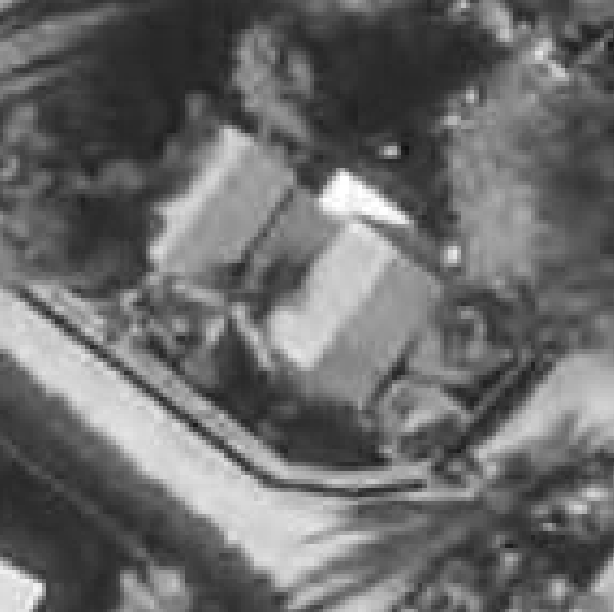
\includegraphics[width=.85\linewidth]{figs/CohBbw.png}
	\caption{\footnotesize{Black and White coherence of image pre-event}}
	\end{subfigure}
	\begin{subfigure}{.475\textwidth}
	\centering
	\captionsetup{width=.85\linewidth}
	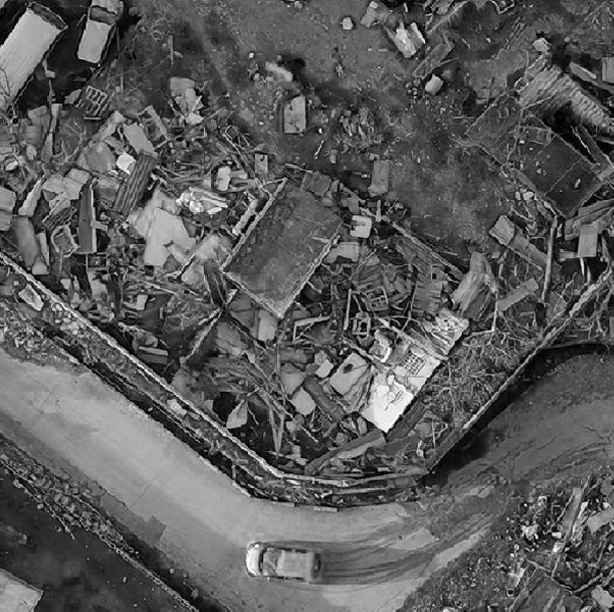
\includegraphics[width=.85\linewidth]{figs/CohAbw.png}
	\caption{\footnotesize{Black and White coherence of image post-event}}
	\end{subfigure}
	\caption{\footnotesize{Structure within an image, pre-event (Left) and post-event (Right) damage sustained [From: Left: IGN France (16 Feb. 2017), Saint-Martin Orthoimage [georeferenced image] | Right: Netherlands Red Cross (15 Sept. 2017), Quilletor Dr - Sint Maarten [georeferenced image] | both used under CC-BY4.0 as part of Open Imagery Network, retrieved from \url{www.openaerialmap.org}]}}
	\label{fig:coh}
\end{figure}

\noindent To identify this structural change \citet{Yun2015} use a equalised coherence maps, one pre-event and one post-event. These maps are created from CSK and ALOS-2 datasets with respective resolutions of 3 meter and 10 meter. Equalisation is achieved through the matching of the histograms of the coherence maps, resulting in statistically equal images in which specific pixel values can vary. Empirically a threshold is chosen to differentiate between noise and change for the detection of damage. Figure \ref{fig:yun}, shows all steps of the process. The results from this approach are used by various agencies around the world, as it allows for a quick visual overview of the damage sustained in a disaster, which can be used for prioritisation of humanitarian aid. The damage sustained is not quantified or projected on [building] features, which limits the process to the interpretation of a user.

\begin{figure}[!h]
	\centering
	\captionsetup{justification=raggedright,singlelinecheck=false}
	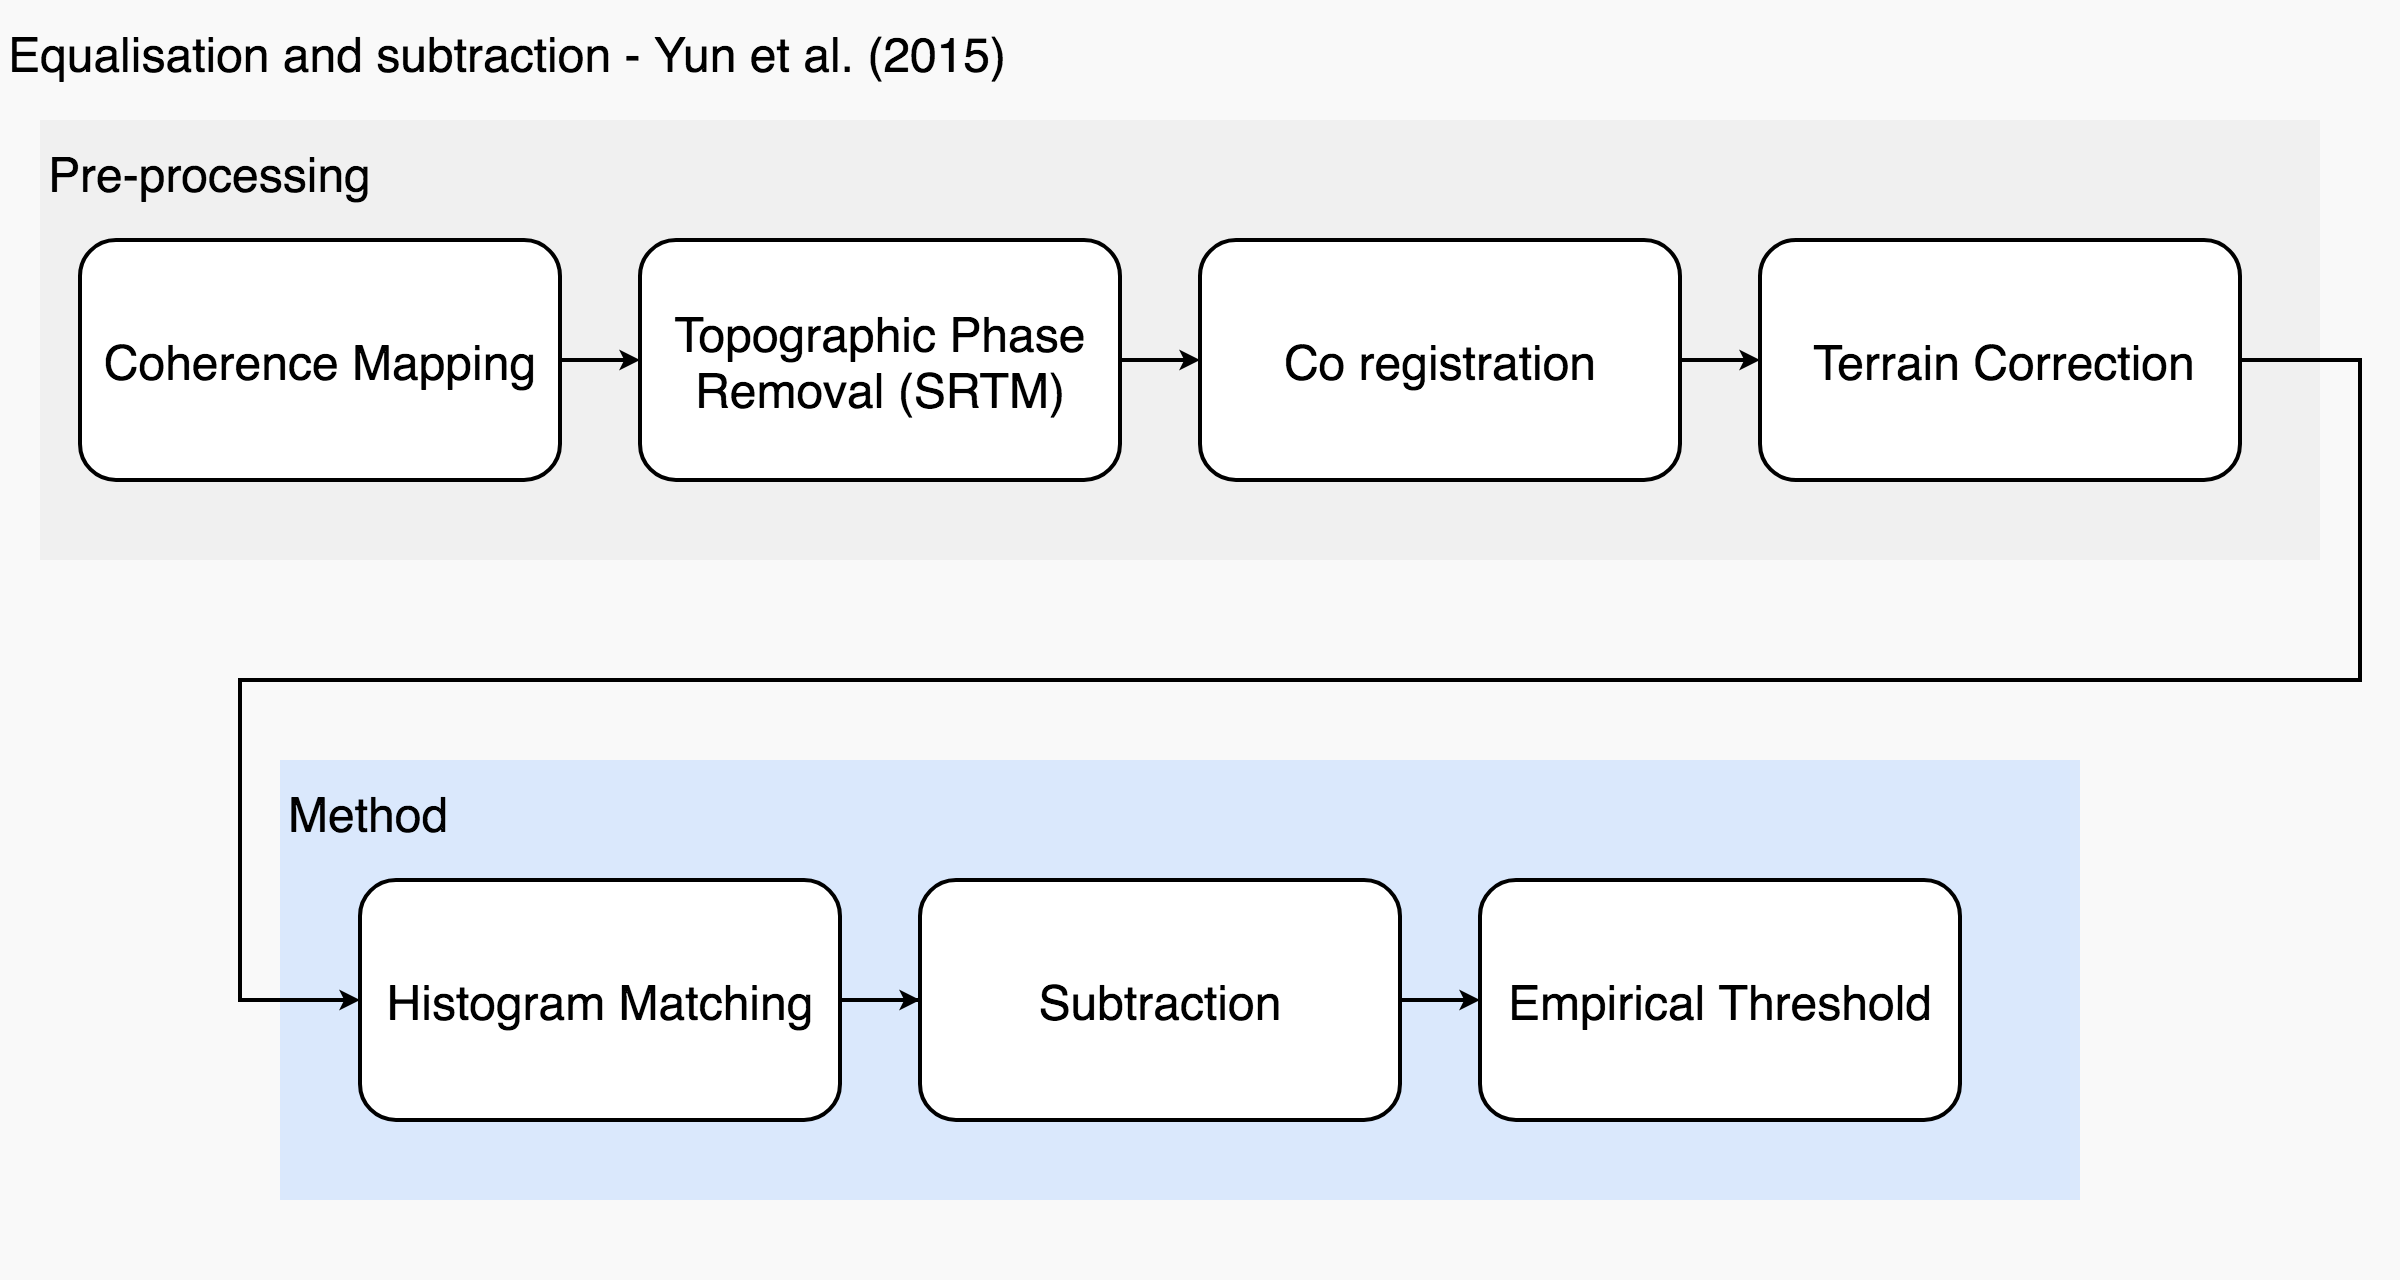
\includegraphics[width=0.95\textwidth]{figs/Yun.png}
	\caption{\footnotesize{Method used by \citet{Yun2015}}}
	\label{fig:yun}
\end{figure}

\subsubsection*{InSAR and Coherence}
Satellite \ac{insar} is a particular use of radar, namely \ac{sar}. Radar makes use of electromagnetic pulses in the microwave spectrum, therefore it is considered an active imaging sensor \citep{Hanssen2001, Ferretti2007}. These properties make it extremely valuable for the imaging of the earth in sub-ideal conditions [night-time or under cloud cover]. As described in section \ref{sec:framework}, time is of the essence in a disaster situation, the ability to gather data under sub-ideal conditions is extremely beneficial for a humanitarian mision. \ac{insar} uses two observation of the same part of the earth to calculate the interferometric observations \citep{Ferretti2007}. These images have a slight offset, which can be achieved by either using two sensors, spatially offset from each other on the same carrier, or the same platform observing the same area twice. This multiplication of the phases of either observation can be used for various remote sensing applications, most notably the generation of a \ac{dem}, or the deformation of the sensed area.\\

\noindent A coherence map is a product derived from the interferometric observation of earth in which the cross-correlation of the phases of either observation is estimated over a kernel \citep{Hanssen2001, Ferretti2007}. The normalised value is a indication of coherence between observations, which can be used for the estimation of noise in observations, as well as change detection. Areas with little to no coherence can usually be correlated to vegetation or other natural environments in which change is observed between offset observations. Man-made structures are related to a high coherence as these are likely to remain similar over larger time spans or various angles. 
 
\subsubsection*{Change detection}
For the detection of change between two images various solutions have been developed over the years based on different approaches \citep{Singh1989, Tewkesbury2015}. \citet{Yun2015} have chosen for a pixel based approach. This Univariate image differencing [equation \ref{eq:singh}] subtracts one observation from the other and transforms these to a positive number \citep{Singh1989}. It is however noted that the threshold chosen for the detection or classification of change influences the outcome of this approach. Various methods for esthablishing the threshold have been developed, ranging from empirically set thresholds to the assessment of the meta-data and various specifics of the images used \citep{Singh1989}. \citet{Yun2015} use an empirically set threshold, in which ground truth data can be used to adjust this parameter.

\begin{equation}
Dx_{ij}^k = x_{ij}^k(t_2) - x_{ij}^k(t_1) + C
\label{eq:singh}
\end{equation}
 
\subsection{Convolutional Neural Network - \cite{Vetrivel2016b}} \label{sec:vet}
\citet{Vetrivel2016b} describe a broad approach to the detection of building damage through the use of machine learning, \ac{cnn} and Support Vector approaches. Their method is tested on various earthquake datasets, i.a. 2010 Port-au-Prince Haiti, 2012 Mirabello Italy, 2015 Kathmandu Nepal. Their proposed method is a comprehensive approach using oblique \ac{uav} imagery. Various characteristics of the imagery are used in the approach which mainly relate to the use of 3D point-cloud features. Oblique imagery allows for the creation of 3D point clouds through a photogrammetric process. The fusion of this point cloud with the imagery is the bases for a Support Vector Classification of the damage. However, in the design process various other methods using machine learning have been tested with varying results, the most promising is the detection of damage features using \ac{cnn}.\\

\noindent Three approaches to the use of \ac{cnn} have been defined by \cite{Vetrivel2016b}. The first approach is the definition of a new \ac{cnn} and training from scratch. For this method the architecture [figure \ref{fig:vet1}] and various settings are provided in the paper. Secondly a pre-trained network from \citet{Krizhevsky2012} has been modified and retrained for the classification of damage. Lastly this retrained network is used for the extraction of features to be used in combination with the 3D point cloud. All \ac{cnn} approaches have been validated for damage detection on the same datasets with respectively 7130 and 5414 classified samples. No significant accuracy increases where found for any of the approaches, all scored within the 90th percentile. These accuracy scores and model transferability quoted in the paper make this a valid approach for similar datasets, in the case of this research ortho-rectified imagery.

\begin{figure}[!h]
	\centering
	\captionsetup{justification=raggedright,singlelinecheck=false}
	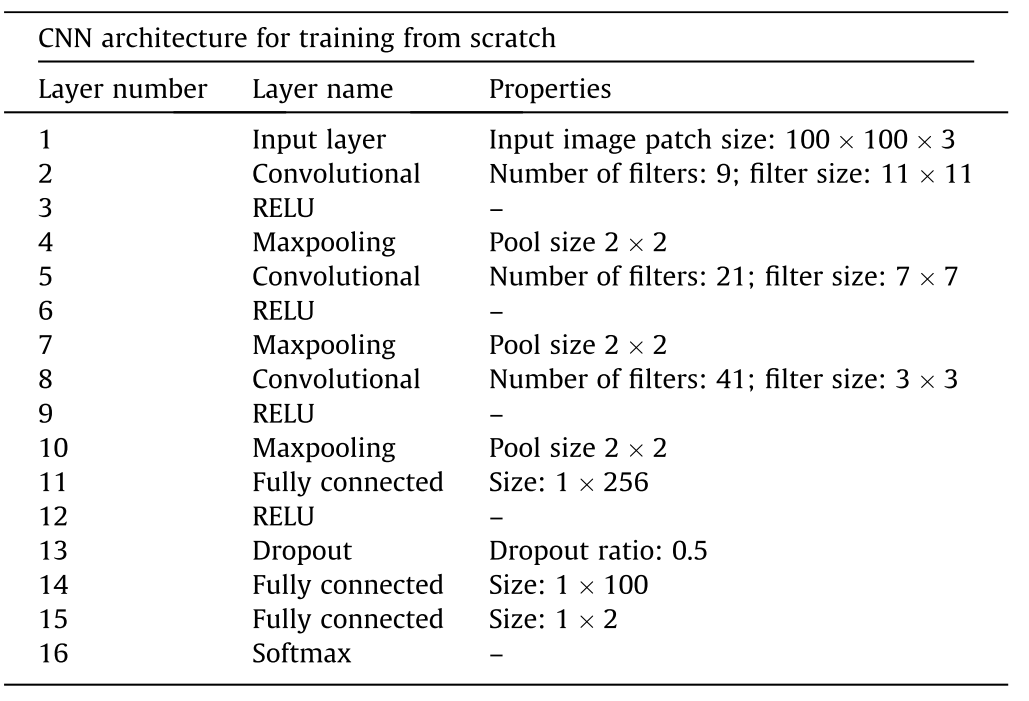
\includegraphics[width=0.95\textwidth]{figs/vet1.png}
	\caption{\footnotesize{CNN architecture [From: \citet{Vetrivel2016b}]}}
	\label{fig:vet1}
\end{figure}

\noindent Due to the various restrictions of this research only one approach to \ac{cnn} for damage detection will be considered. As there are no accuracy benefits for choosing any, other circumstances will be taken into consideration. The simple approach to a new \ac{cnn}, which can be trained from scratch will guarantee the model awareness of the data, increasing the changes of correct classification. A similar sized training set is available and the new approach allows for fine-tuning. The steps necessary to achieve an approach as described by \citet{Vetrivel2016b} is summarised in \ref{fig:vet2}.

\begin{figure}[!h]
	\centering
	\captionsetup{justification=raggedright,singlelinecheck=false}
	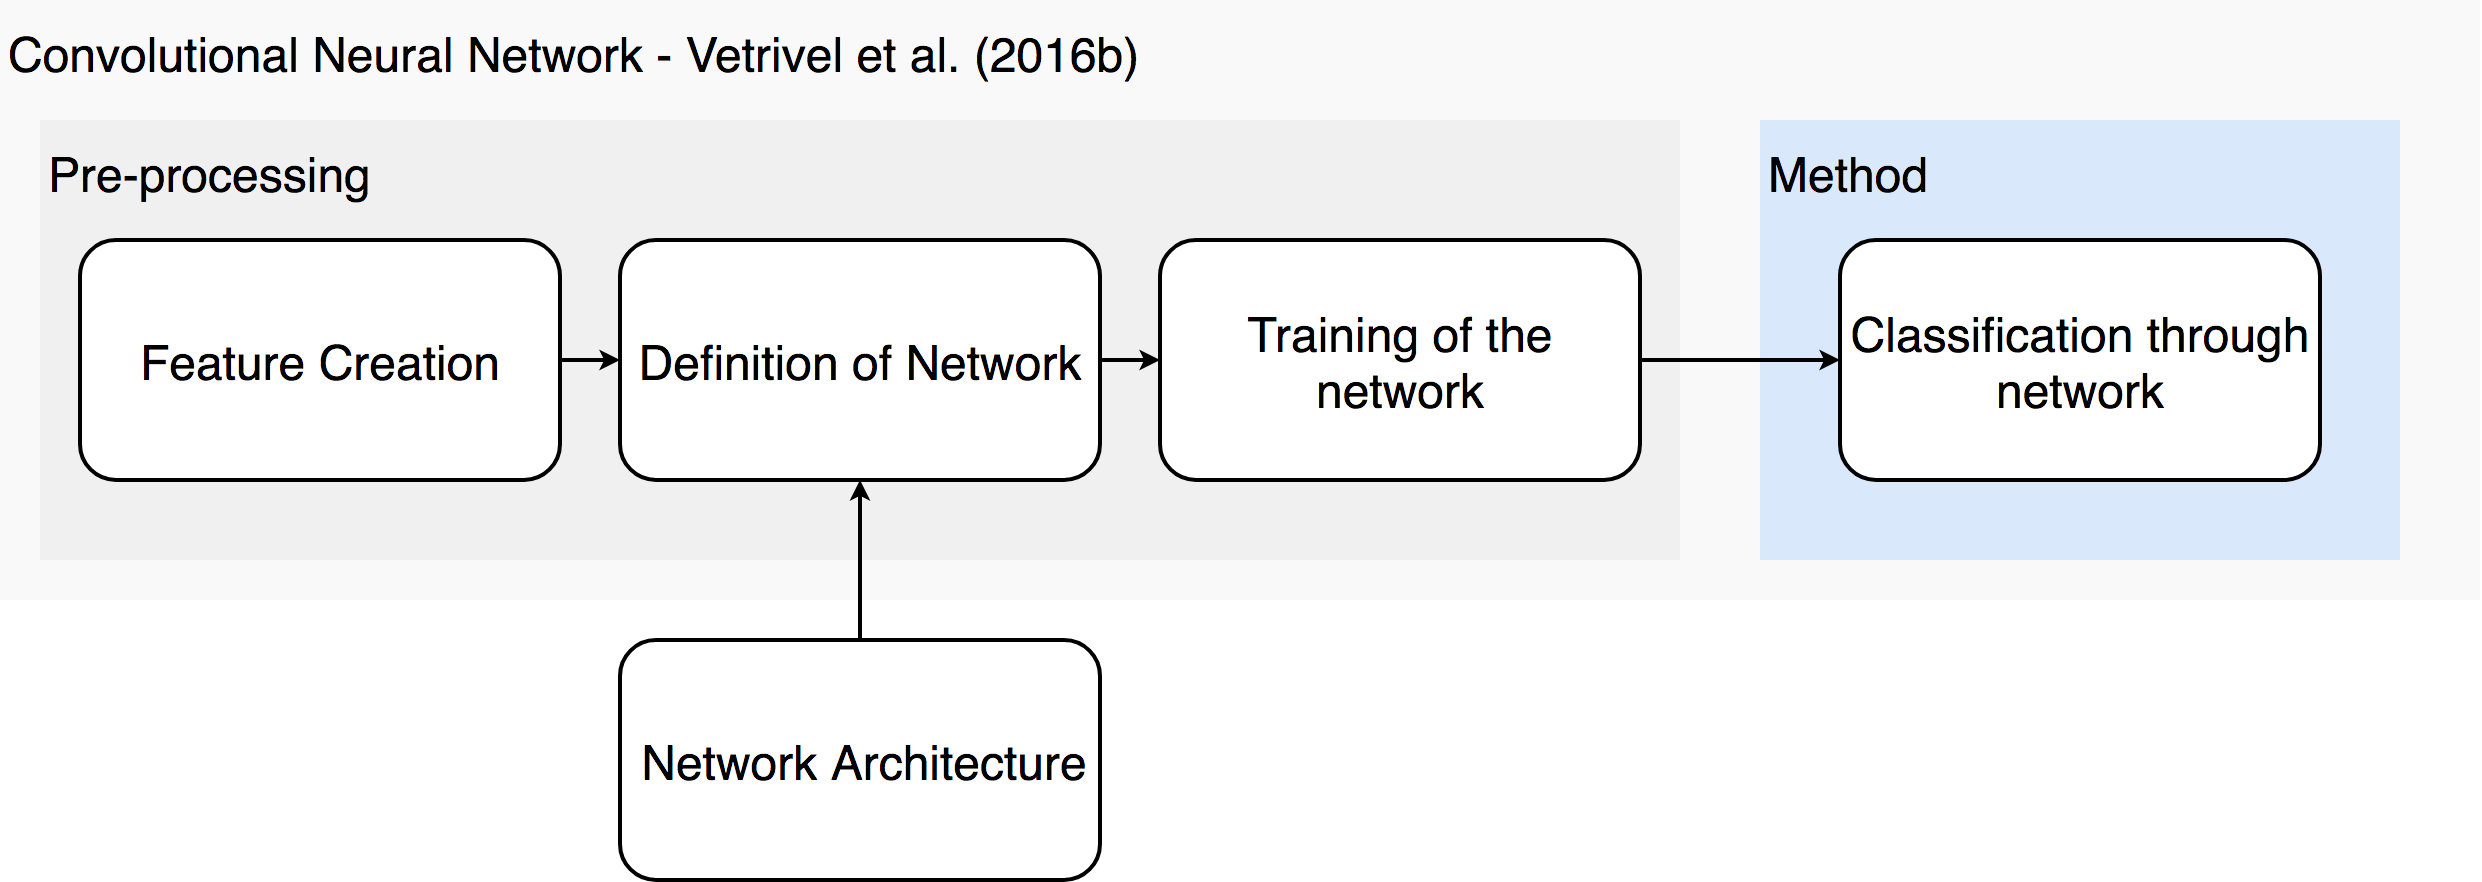
\includegraphics[width=0.95\textwidth]{figs/vet2.png}
	\caption{\footnotesize{\ac{cnn} implementation from scratch, \citet{Vetrivel2016b}}}
	\label{fig:vet2}
\end{figure}

\subsubsection*{Neural network}
Neural networks, and therefore also \ac{cnn}s, have come from the field of deep learning \citep{Hardesty2017}. This approach to machine learning is roughly modelled on the human brain. A network of connections is being trained to perform a specific task, for example the classification of data. The first mentions of such an approach to machine learning date back to the second half of the last century \citep{Lawrence1997, Hardesty2017}. \ac{cnn}s have evolved to become a distinct approach within Neural Networks, in which various layers guide data through filters to reduce data and deduct weights and thresholds. A simple \ac{cnn} has been shown in figure \ref{fig:NN}, in which the various convolutional layers reduce the images by kernels, activated with a specific algorithm. These so-called pooling algorithms are used to reduce the data. This pyramid structure allows the last layer, usually a regression algorithm, to determine the class assigned to the specific feature \citep{Lawrence1997}.

\begin{figure}[!h]
	\centering
	\captionsetup{justification=raggedright,singlelinecheck=false}
	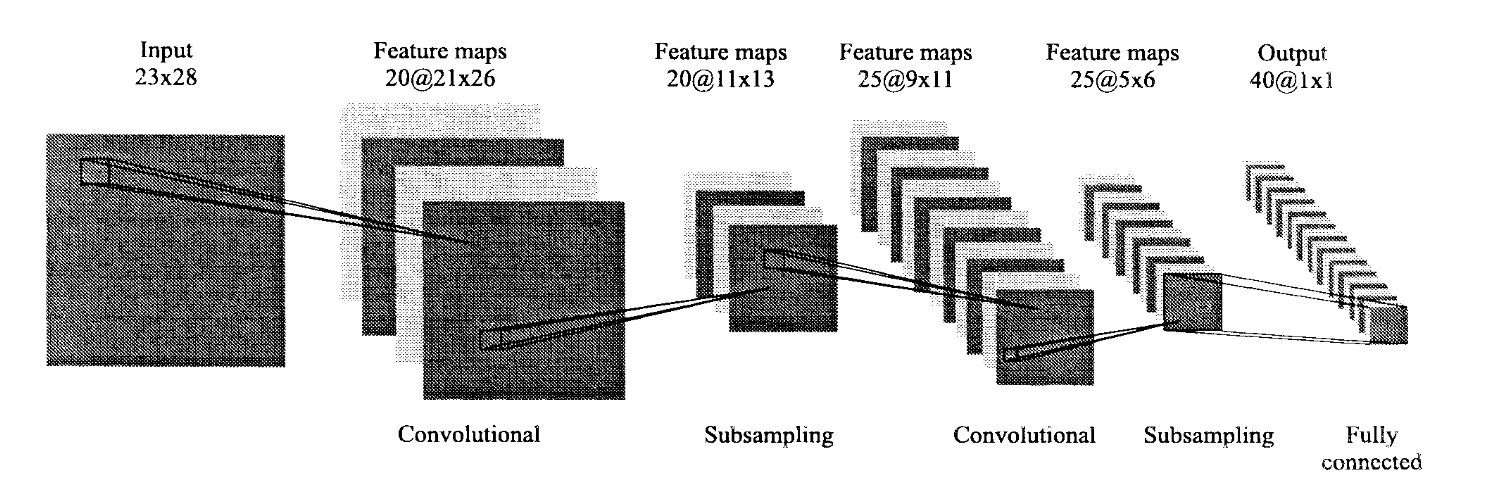
\includegraphics[width=0.95\textwidth]{figs/nn.png}
	\caption{\footnotesize{A simple \ac{cnn}. [From: \citet{Lawrence1997}]}}
	\label{fig:NN}
\end{figure}

\section{Related background information} \label{sec:relb}
\subsection{Colour space}
For the comparison of approaches as mentioned in section \ref{sec:met}, various colour spaces are used to gain a simplification of the dataset. Colour spaces are methods used for standardisation of the description of colour. These are all based around the sensations regarding colour perception as described by \citet{Hunt2011, ford1998colour}. These are:\\
\begin{itemize}
	\item Brightness of a colour, regarding the variance in light
	\item Hue of a colour, the similarity between colour, usually expressed in \ac{rgb}
	\item Colourfulness of a specific area, the amount of hue in a feature
	\item Lightness, this is a description of brightness referenced to a white area
	\item Chroma, is the colourfulness referenced to lightness
	\item Saturation, is the colourfulness relative to the brightness.\\
\end{itemize}

\noindent\citet{ford1998colour} describe the various colour spaces available for use. These are all used for various applications and are simplifications of the sensations of colours for humans. These simplifications are necessary for computers to represent colours as data. The colour spaces considered in this research are \ac{rgb} and \ac{hsl}, specifically \ac{hsv}. \ac{rgb} is the most commonly used colour space, most cameras and monitors represent colour in this way \citep{ford1998colour}. It separates the colour into 3 bands described by Red, Green, and Blue, while all other colours are a mix of these 3. It is easy to implement and understand [figure \ref{fig:rgb}], but are non-linear with human sensations of colours. \ac{hsl} is a group description for colour spaces in which the first two parameters are Hue and Saturation, while the last is on of the other options for sensations of colour as described in the list above. For this research \ac{hsv} has been chosen. Value is used to describe the colourfulness of an area [figure \ref{fig:hsv}]. As \ac{rgb} these colour spaces are non linear, and can therefore be linearly transformed both ways using pseudo-code as described by \citet{schwarz1987} [Code block \ref{code:colour}]. However, they are more intuitive and comparable to the sensation of colour for humans. This comparability allows for introduction into the classification process of damage. Visual interpretation is the preferred method used for damage detection [chapter \ref{intro}] and a more comparable approach to colour definition could help the introduction of automated approaches. \ac{hsv} is more computationally effective than \ac{hsl} and has therefore been applied in this research \citep{schwarz1987}.\\

\begin{figure}[!h]
	\centering
	\begin{subfigure}{.475\textwidth}
		\centering
		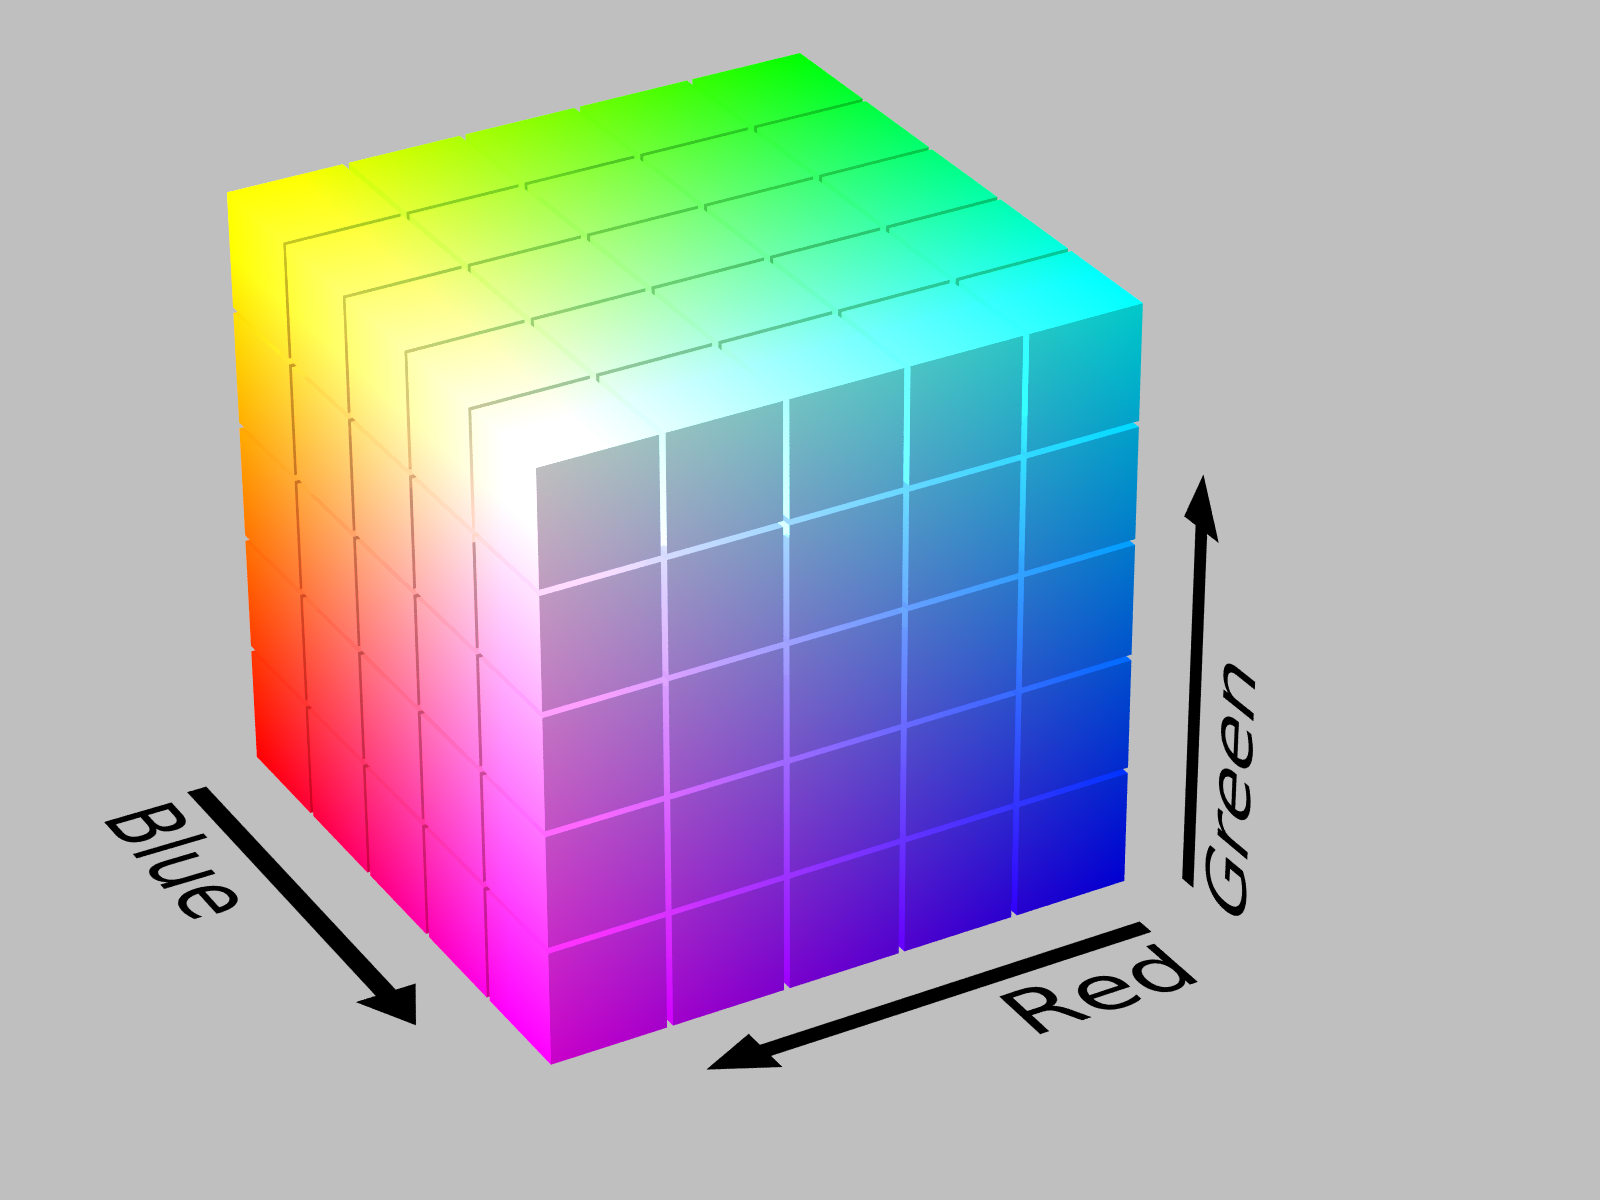
\includegraphics[width=.8\linewidth]{figs/RGB_Cube.png}
		\caption{\footnotesize{\ac{rgb} colour space}}
		\label{fig:rgb}
	\end{subfigure}
	\begin{subfigure}{.475\textwidth}
		\centering
		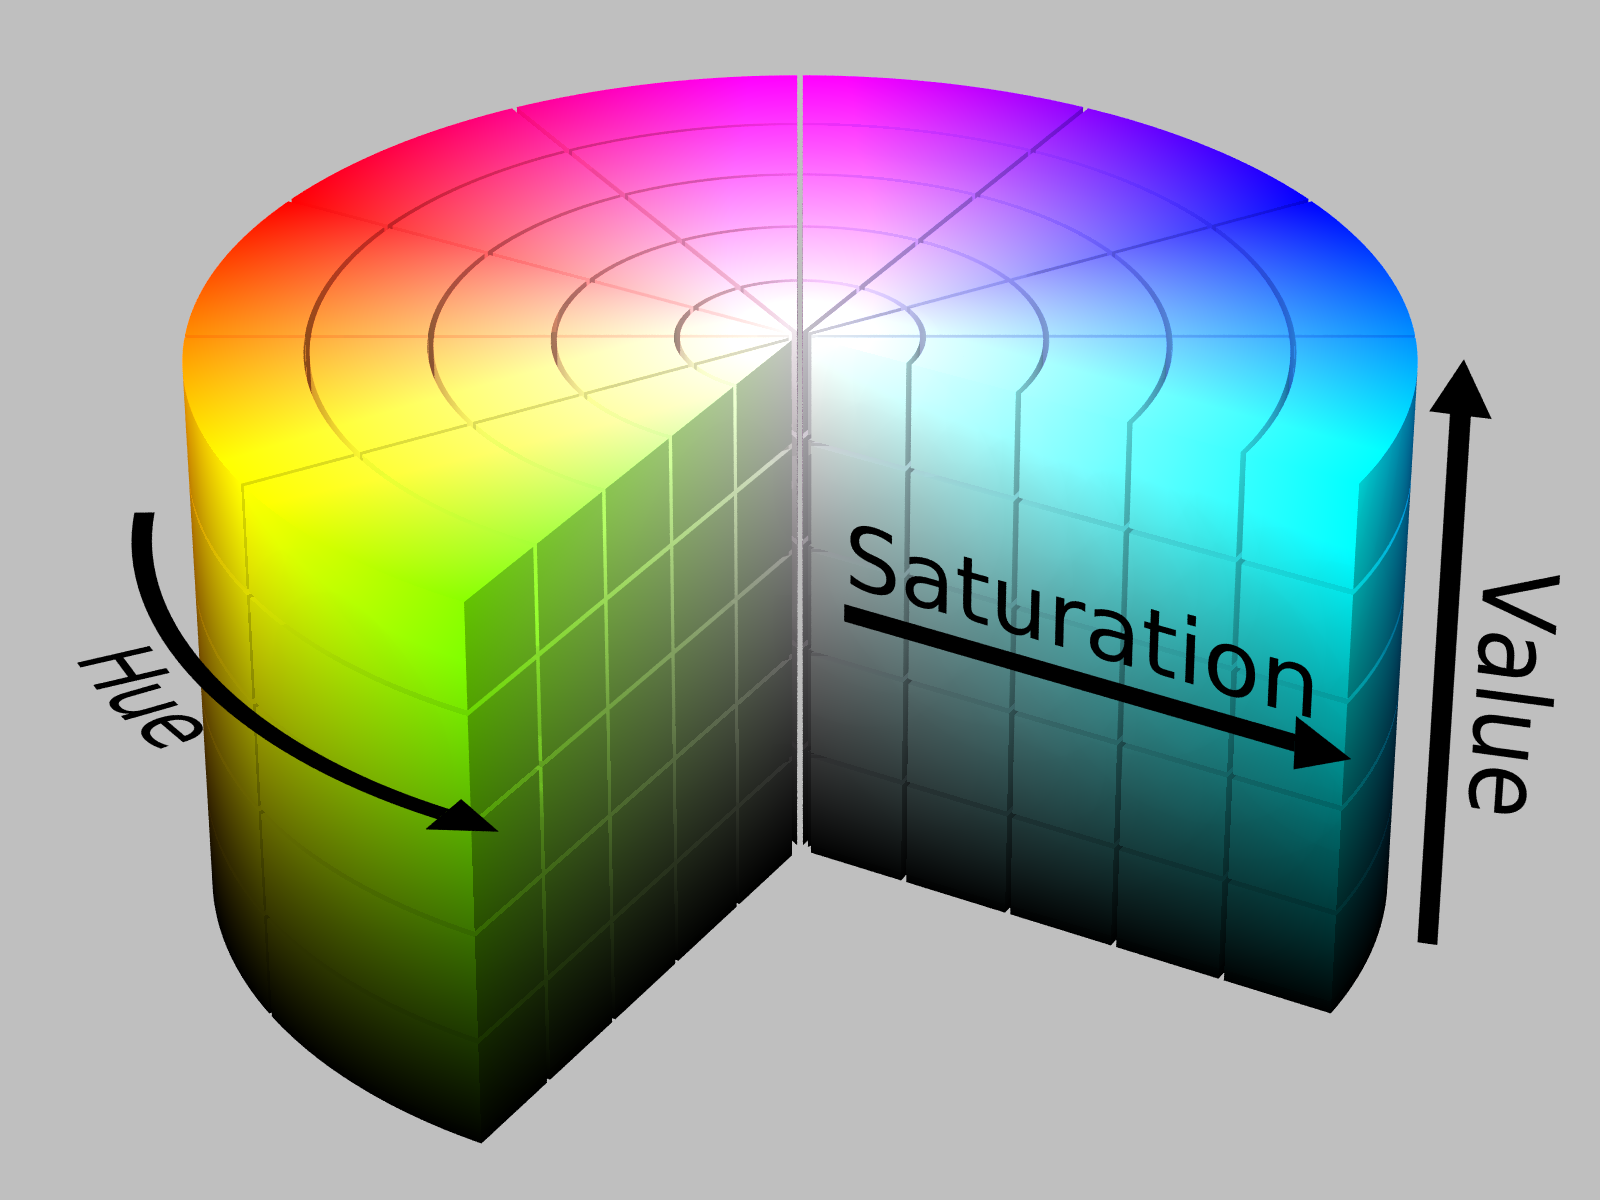
\includegraphics[width=.8\linewidth]{figs/HSV_color.png}
		\caption{\footnotesize{\ac{hsv} colour space}}
		\label{fig:hsv}
	\end{subfigure}
	\caption{\footnotesize{Colour spaces visualised in 3D. [From: \citet{Horvath2011}]}}
	\label{fig:colourspace}
\end{figure}

\begin{equation}
	\begin{split}
		&\text{Psuedo code \: \ac{rgb} \: to \: \ac{hsv} \: from \: \citet{schwarz1987}}
		\\
		&F = H * 6 - Floor(H*6) \\
		&T_1 = V * (1.0 - S) \\
		&T_2 = V * (1.0 - (S * F)) \\
		&T_3 = V * (1.0 - (S * (1.0 - F))) \\
		\\
		&case\: floor(H*6)\: mod\: 6\: of\\
		&\qquad 0: (R,G,B) = (V, T_3, T_1)\\
		&\qquad 1: (R,G,B) = (T_2, V, T_1)\\
		&\qquad 2: (R,G,B) = (T_1, V, T_3)\\
		&\qquad 3: (R,G,B) = (T_1, T_2, V)\\
		&\qquad 4: (R,G,B) = (T_3, T_1, V)\\
		&\qquad 5: (R,G,B) = (V, T_1, T_2)\\
	\end{split}
\label{code:colour}
\end{equation}

\subsection{Inter-rater statistics} \label{sec:interrater}

Cross classification is a popular statistic to describe the accuracy of a method for prediction \citep{Warrens2011}. The description of these inter-rater statistics have been developed throughout many academic fields. These have originally been developed to determine the accuracy of two human raters in various research fields \citep{Bhowmick2008}. However, with the growth of machine learning and other predictors, these indices have been used more to describe their performance with regards to ground truth. This more elaborate description of cross classification or inter-rater statistics is used in this field to compensate for the possibility of unbalanced input and outcomes, in which a larger subset of a specific class might affect the accuracy, in which only the correct answers are considered [Equations \ref{eq:acc}]. \\

\begin{equation}
\begin{split}
&\text{accuracy} = \frac{\text{correctly classfied samples}}{\text{total classified samples}} \\
\end{split}
\label{eq:acc}
\end{equation}

\noindent For this research, two methods to describe inter-rater statistics have been chosen. These are the so-called F1-score [Sørensen–Dice coefficient] and the Cohen Kappa coefficient \citep{Dice1945,Sorensen1948,Cohen1960}.Both of these are popular and established methods for the description of inter-rater accuracy for the evaluation of learning algorithms.

\subsubsection*{Cohen Kappa}
The Cohen Kappa is developed in 1960 by Jacob Cohen at New York University \citep{Cohen1960}. It's first implementation was used to describe the categorisations [nominal descriptors] of 2 observers in clinical-social-personality studies. The kappa score is described by \cite{Cohen1960} as an indicator of agreement. In the definition of the Cohen Kappa coefficient, it compares the agreement between observers compared to random assignment \citep{Warrens2011}. From which the statistic can handle imbalances between classes as well as multiple classes \citep{Kampakis2016}. These characteristics make it useful for the description of performance in nominal machine learning techniques, and therefore a suitable descriptor for the performance of the methods considered in this research.\\

\noindent As described by \citet{Warrens2011}, the Cohen Kappa coefficient is given in equation \ref{eq:kappa}. Which holds true if the categories are in the same order for both observers, such that the row and column totals can be described as in equation \ref{eq:col}.
\begin{equation}
	\begin{split}
		&\kappa = \frac{P - E}{1 - E} \\
		&\text{Where} \\
		&P = \sum_{j=1}^{n} p_{jj} \quad\text{and}\quad E= \sum_{j=1}^{n} p_jq_j \\
	\end{split}
	\label{eq:kappa}
\end{equation}

\begin{equation}
	\begin{split}
		&p_j = \sum_{k=1}^{n} p_{jk}  \quad\text{and}\quad q_j = \sum_{k=1}^{n} p_{kj}
	\end{split}
	\label{eq:col}
\end{equation}

\subsubsection*{F1-Score}
The F1-score or Sørensen–Dice coefficient is based on the work of \citet{Dice1945}, in which the association between species is measured, and \citet{Sorensen1948}, in which the same is described for plants. This method considers the harmonic mean of both recall and precision \citep{Sasaki2007}. In this descriptor of inter-rater statistics, the precision is considered the rightly classified as proportion of the total classified within one category; recall is considered the inverse of precision as described as the proportion of the rightly classified over the ground truth total within one category \citep{Buckland1994}. This description was generalised by \citet{Chinchor1991} in which the classifier could be varied by an $\beta$ constant. As described by \citet{Sasaki2007}, the F1-score reflects to $\beta = 1$, with a resulting equation \ref{eq:f1}, in which $P$ is precision and $R$ is recall.

\begin{equation}
\begin{split}
&F=\frac{2PR}{P+R}
\end{split}
\label{eq:f1}
\end{equation}

\noindent The development of this method for cross classification in information retrieval by \cite{Chinchor1991} and the broader statistics of the data with the inclusion of precision and recall per category, allow for an in-depth understanding of the results of machine learning algorithms. These characteristics suit this research, as it provides more understanding of the results per classification category than the generalised Cohen Kappa coefficient. The inclusion of the other precision and recall indicators is, however, paramount.

\subsubsection*{Critique on inter-rater statistics}
Both the F1-Score and Cohen Kappa coefficient are not unscrutinised \citep{Feinstein1990, Pontius2011, Powers2015}. The use of Cohen Kappa leaves some room for ambiguity, however is still the most accurate method to measure agreement while factoring in random assignment. It can however be bias in some extremely unbalanced test sets in which the categories are skewed to a particular classification. As described by \citet{Powers2015}, the F1-Score should only be used to look at one category at a time, this because it is very sensitive to majority classes. A balance between methods is therefore necessary. The inclusion of recall and precision can be used to further explain the Cohen Kappa coefficient, while taking into account limitations from both methods.